\section{Interaktion der Komponenten}
Auf Basis der Analyse Use Cases wird in diesem Kapitel die Interaktion der einzelnen Komponenten aus Kapitel 1 betrachtet. Dabei liegt der Fokus vor allem der Interaktion zwischen dem Server und der RobotUnit. Die Use Cases innerhalb der Komponenten werden in Kapitel 8 näher ausgeführt. \\


\subsection*{Interaktion bei Ausführung von \emph{Take Patient To Hospital}}

Zuallerst fragt das Hospital über Check availability (Use Case 8) den Server an, ob ein Roboter überhaupt verfügbar ist. Dann läuft die Auswahl eines Robots wie im Diagramm beschrieben folgendermaßen ab: Bei einer neueingehenden Destination sendet der Server mit getSensorData(task) Anfragen an alle zur Verfügung stehenden RobotUnits(, im Diagramm sind Beispielhaft zwei angeführt, der Aufruf findet asynchron statt.) Die RobotUnit führt dann Read Sensor(Use Case 3) aus. Dabei sammelt er alle notwendigen Informationen von seinen Hardwareschnittstellen, wie Ladestand und Nähe zum Ziel, die der Server benötigt um den bestmöglichen Roboter auszuwählen. Er wartet auf das Zusammentragen der Daten, also das Abschließen des internen Loop-Prozesses, bis er eine Nachricht mit den Informationen an den Server zurücksendet; erst dann kann der Server auf Grund der übermittelten Daten beurteilen, welcher Roboter am besten geeignet ist den Patienten abzuholen(demzufolge das beste rating hat) und entsendet ihn zu den Zielkoordinaten( Usecase 7 Assign Task.) Nicht mehr in der Abbildung beschrieben ist dann der Uscase Inform about borading (Usecase 9), da er keinen unmittelbaren Teil des Select Best Match Prozesses bildet. Sobald der Roboter den Patienten erreicht und dieser sicher auf ihm verladen wurde, meldet das Hospital dies unverzüglich über dem Server an den Roboter zurück. Im Gegenzug existiert ebenso der Use Case Inform about arrival(Usecase 5): Bei dem der Roboter sobald er das Krankenhaus erreicht hat, die Information an den Server weiterleitet, um die bestmögliche Koordinate über den Server mit dem Krankenhaus zu ermöglichen und die Versorgung des Patienten sofortig zu gewährleisten.

Bei den weiteren UseCases ist der Server nicht beteiligt. Das schließt auch den UseCase Charching(Use Case 4) ein. Dort kommt es ausschließlich zur Wechselwirkung mit der CharchingStation Komponente.


\begin{figure}[H]
	\centering
	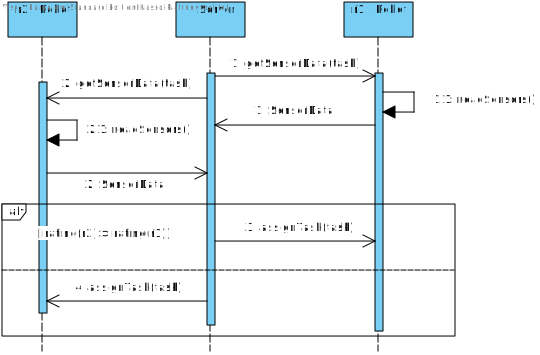
\includegraphics[width=0.9\textwidth]{img/0-Entwurf-2-ChooseRob}
	\caption{\emph{ChooseRobot}-Sequenzdiagramm}
	\label{SequenzDiagrammInteraktion}
\end{figure}
